\section{Einführung}
Roomba Kart ist ein an Mario Kart angelehntes Rennspiel, welches von zwei Spielern gegeneinander gespielt werden kann. Die Karts sind zwei umfunktionierte Staubsaugerroboter des Herstellers Roomba. Die Karts werden von zwei Logitech Fernbedienungen gesteuert und sind mit einem Arduino Board, an denen ein Funkmodul angebracht ist, verbunden. Hierdurch können sich die Kontrahenten gegenseitig beeinflussen und dadurch stören. Im Folgenden wird detailiert beschrieben, wie ein Spiel gestartet werden kann, die Steuerung funktioniert und die Regeln lauten. 

\section{Spielstart}
Die mindeste und maximale Anzahl von Spielern, die beim Roomba Kart mitmachen können, ist zwei. Um mitspielen zu können, braucht jeder Spieler einen Roomba, ein mit dem Spiel programmiertes Arduino Board mit Funkmodul und eine Ferbedienung. Das Arduino Board wird durch eine Steckverbindung mit dem Roomba verbunden. Im Anschluss sollten auf dem Roomba-Display vier Bindestriche anzeigt werden. Falls dies nicht der Fall ist, muss der Resetbutton auf dem Arduino Board gedrückt werden.

Durch die vier Bindestriche werden die Spieler aufgefordert anzugeben, ob sie Spieler 1 oder 2 sind. Durch die Eingabe der entsprechenden Ziffer mittels der Fernbedienung und einer Bestätigung der Eingabe durch die Rechtstaste gefolgt von der Powertaste, werden die Spieler festgelegt. Bei einer Fehleingabe wird dies angezeigt und eine erneute Eingabe ist möglich. Die Spieler müssen sich unterscheiden, da sonst keine Funkverbindung zustande kommen kann und unterschiedliche Tasten für die Fernbedienung festgelegt werden, damit die Spieler sich nicht gegenseitig steuern.
   
\section{Steuerung}
Im folgenden werden kurz die allgemeine Steuereigenschaften erklärt. Danach wird die Steuerung für Spieler 1 und im Anschluss die Steuerung für Spieler 2 beschrieben. 

\underline{Allgemein:} 

Das Kart hält selbständig seine Geschwindigkeit. Die Spieler können durch die Vorwärtstaste bzw. Rückwärtstaste Einfluss auf die Geschwindigkeit nehmen und bestimmen, ob das Kart vorwärts oder rückwärts fahren soll. Durch die Rechts- und Linkstaste bestimmt der Spieler, in welche Richtung sein Kart fahren soll. Desto länger die Links- oder Rechtstaste gedrückt wird, desto stärker lenkt das Kart in die jeweilige Richtung. Wenn die Links- oder Rechtstaste nicht mehr gedrückt wird, fährt das Kart wieder selbstständig geradeaus. Eingesammelte Powerups können durch die Schusstaste abgeschossen werden.

\underline{Spieler 1:}

Spieler 1 steuert sein Kart mit dem Steuerkreuz der Fernbedienung und feuert seine Powerups mit der Powertaste ab. Eine detaillierte Beschreibung bietet die folgende Abbildung bzw. Tabelle:

\begin{center}
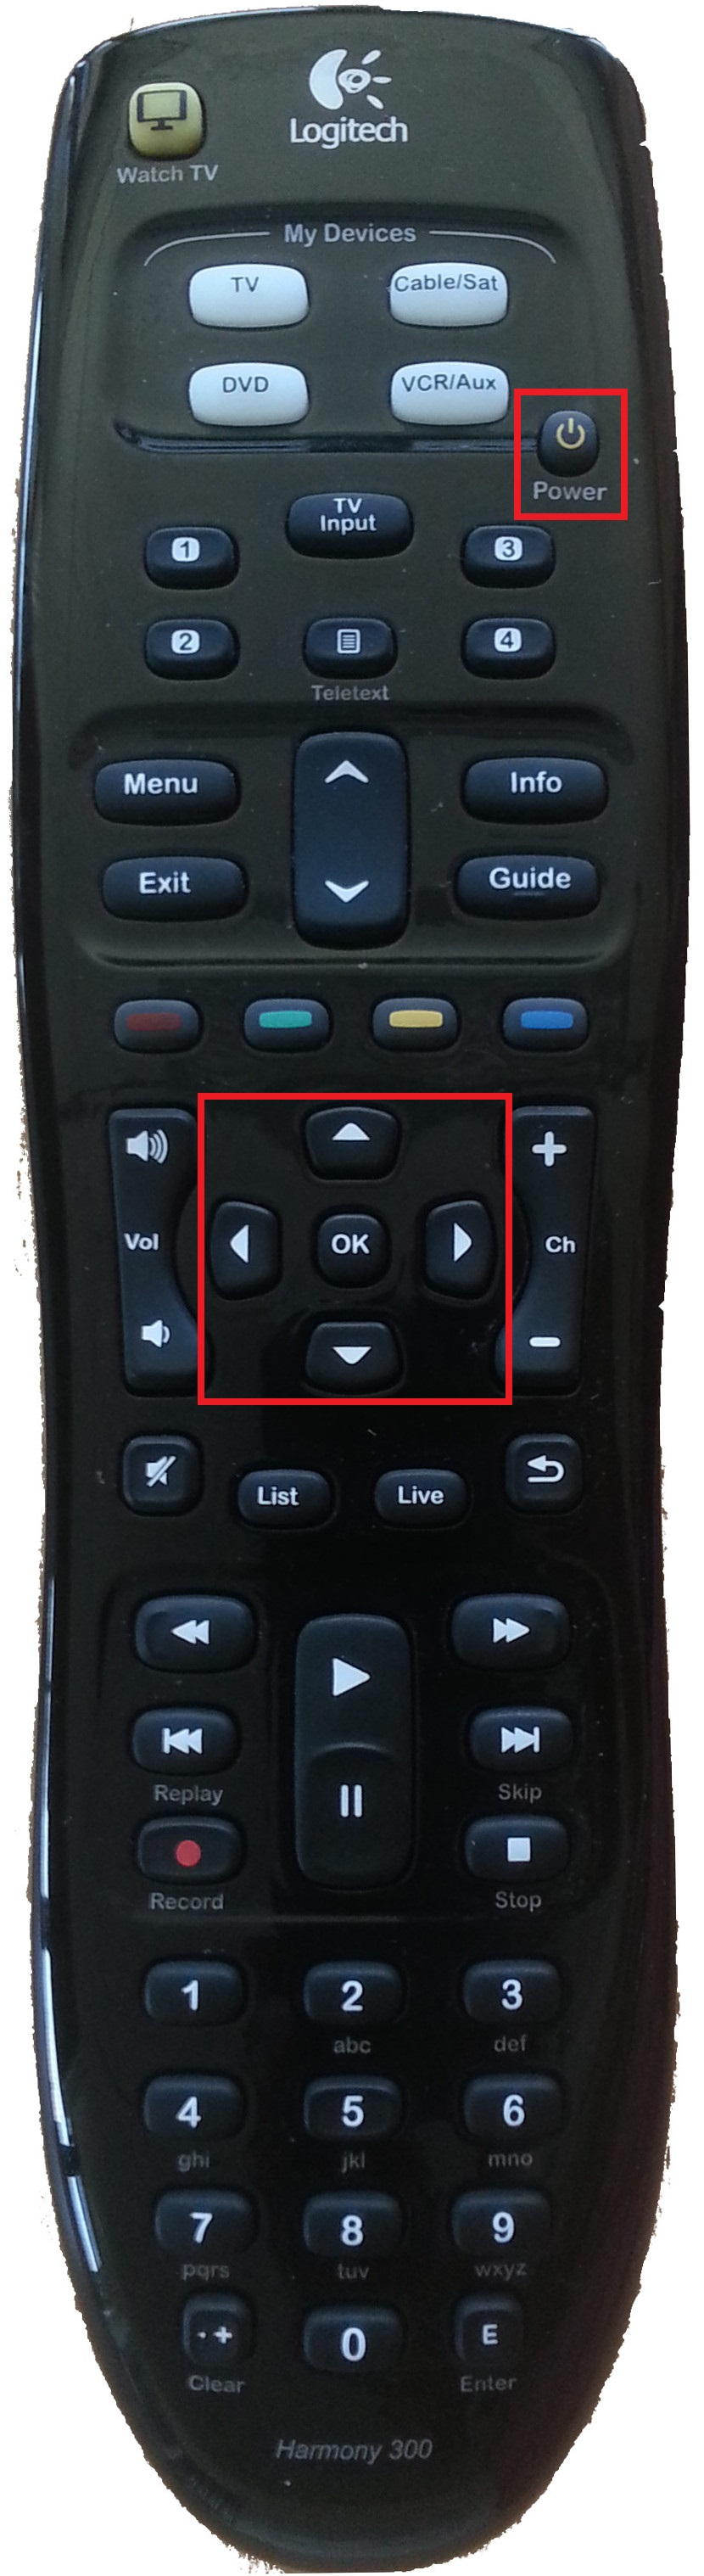
\includegraphics[scale=0.1]{Bilder/Steuerung_Spieler1}
\end{center}

\vspace{0.5cm}
\begin{tabular}{|l|l|}
\hline
\textbf{Taste} & \textbf{Auswirkung} \\ \hline
Steuerkreuz hoch & Vorwärtstaste: Kart beschleunigt \\ \hline
Steuerkreuz runter & Rückwärtstaste: Kart fährt rückwärts/bremst \\ \hline
Steuerkreuz links & Linkstaste: Kart fährt nach links \\ \hline
Steuerkreuz rechts & Rechtstaste: Kart fährt nach rechts \\ \hline
Powertaste & Schusstaste: Kart feuert Powerup ab, falls vorhanden \\ \hline  
\end{tabular} 
\vspace{0.5cm}

\underline{Spieler 2:}
 
Spieler 2 steuert sein Kart mit den Nummerntasten der Fernbedienung und feuert seine Powerups mit der Taste 5 ab. Eine detaillierte Beschreibung bietet die folgende Abbildung bzw. Tabelle:

\begin{center}
	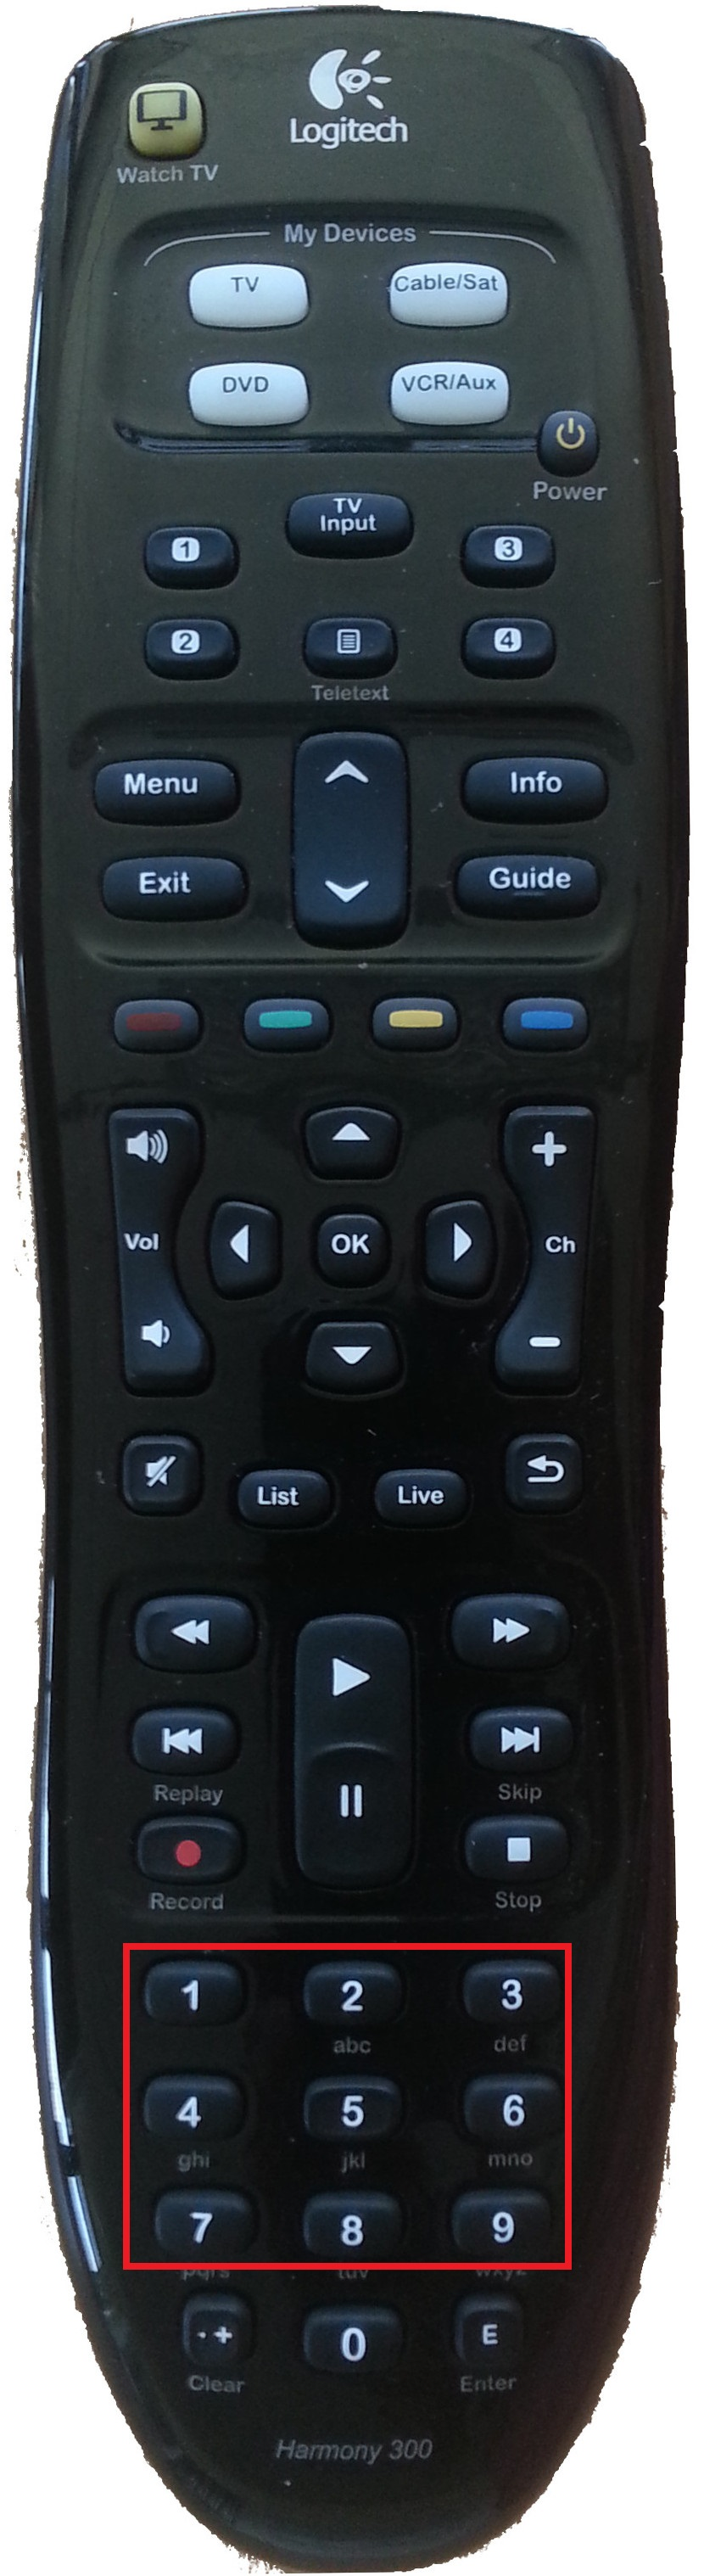
\includegraphics[scale=0.1]{Bilder/Steuerung_Spieler2}
\end{center}

\vspace{0.5cm}
\begin{tabular}{|l|l|}
\hline
\textbf{Taste} & \textbf{Auswirkung} \\ \hline
Taste 2 & Vorwärtstaste: Kart beschleunigt \\ \hline
Taste 8 & Rückwärtstaste: Kart fährt rückwärts/bremst \\ \hline
Taste 4 & Linkstaste: Kart fährt nach links \\ \hline
Taste 6 & Rechtstaste: Kart fährt nach rechts \\ \hline
Taste 5 & Schusstaste: Kart feuert Powerup ab, falls vorhanden \\ \hline 
\end{tabular}
\vspace{0.5cm}

\section{Regelwerk}
Ein Rennen zwischen zwei Kontrahenten dauert fünf Runden. Sieger ist derjenige, der den im Embeddedlabor aufgebauten Kurs zuerst fünf mal erfolgreich absolviert hat. Die Richtung spielt hierbei keine Rolle. Das bedeutet, dass der Kurs sowohl in die eine als auch in die andere Richtung gefahren werden kann. Bei Uneinigkeit zwischen den Kontrahenten, muss eine Strafrunde absolviert werden. Falls nachweislich betrogen wurde, erfolgt die sofortige Disqualifikation oder Verlust des Titels und eine dreijährige Sperre. 

Ein vorsetzliches oder versehentliches Verlassen des Parcours wird bestraft. Die Bestrafung äußert sich dadurch, dass sich das Kart kurzeitig selbständig fährt und sich zurück in die Mitte der Fahrbahn manövriert. Dieser Vorgang kostet wertvolle Sekunden, die der Gegner zum Überholen bzw. Aufholen nutzen kann. Damit die Erkennung des Streckenrands und das korrekte hereinfahren in die Mitte des Kurses funktioniert, sollte die Streckenbegrenzung drei Lagen Klebeband breit sein. Der Mechanismus des Zurück-Fahrens funktioniert dabei folgendermaßen: Erkennt ein vorderer Cliff-Sensor ein Klebeband, merkt sich der Roboter, ob der linke oder rechte Sensor aktiv wurde, um später entscheiden zu können, in welche Richtung er innerhalb der Strecke drehen muss. Sind beide vorderen Sensoren aktiv, erkennt der Roboter, dass er auf dem Klebeband ist und stoppt. Anschließend fährt das rechte Rad solange rückwärts, bis der seitliche Cliff-Sensor ein Klebeband entdeckt. Da sich die Sensoren nicht auf der Radachse befinden, wird nun jeweils nocheinmal links und rechts nachkorrigiert, bis beide seitlichen Sensoren ein Klebeband erkennen – das heißt, der Roboter im $90^\circ$ Winkel zur Streckenbegrenzung steht. Anschließend fährt der Roomba 30 Zentimeter gerade aus und dreht sich um $90^\circ$, um wieder streckenparallel zu stehen (Richtung abhängig vom zuerst aktiven Sensor s.o.).

Falls ein Spieler den gegnerischen Spieler, das gegnerische Kart oder ein anderes Hindernis rammt (Bump-Sensoren aktiv), fährt das andere Kart solange mit einer erhöhten Geschwindigkeit, bis sein Pilot durch drücken einer Steuertaste eingreift. Dieser Vorgang kann bei riskanten Überholmanövern in der Endphase über Sieg oder Niederlage entscheiden. Diese Information (und der gegnerische Abschuss) wird über das Funkmodul übertragen. Es wird dabei maximal drei mal versucht, die Information zu übertragen und auf ein ACK-Signal zu warten. 

Speziell in Alufolie gekleidete Powerup-Stations am Streckenrand dienen der Generierung von Powerups. Ein Sensor vorne rechts im Kart (Wall-Sensor) registriert diese bei sehr nahem Vorbeifahren. Im Anschluss wird durch einen Zufallsgenerator ein Powerup ausgewählt. Ist bereits ein Powerup aufgesammelt, bzw. gerade aktiv, kann kein neues Powerup gesammelt werden. Powerups können bei sinvollem Gebrauch wertvolle Zeit verschaffen bzw. den Gegner stark beeinträchtigen. Ein Powerup das auf das gegnerische Kart abgefeuert wird, ist nicht wirksam, wenn dieses gerade eine automatische Kurskorrektur vornimmt. Folgende Powerups sind verfügbar: 

\begin{itemize}
	\item RED TANK: Wird als kleiner Panzer auf dem Display des Karts angezeigt:
	
	\begin{center}
		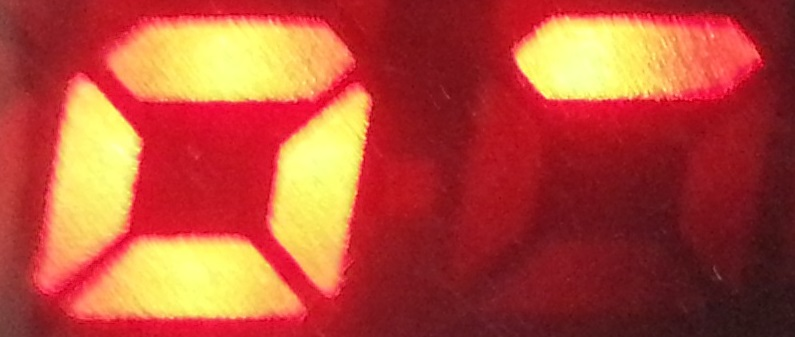
\includegraphics[scale=0.3]{Bilder/RED_TANK}
	\end{center}
	
	Wirkung: Wenn dieses Powerup abgeschossen wird, dreht sich das gegnerische Kart um $1080^\circ$. Ein verfehlen ist nur dann möglich, wenn sich der gegnerische Spieler rechtzeitig durch das Powerup BIG DADY schützt. Ein evtl. gesammeltes Powerup des getroffenen Spielers geht verloren und auf dem Display erscheint HIT:
	\begin{center}
		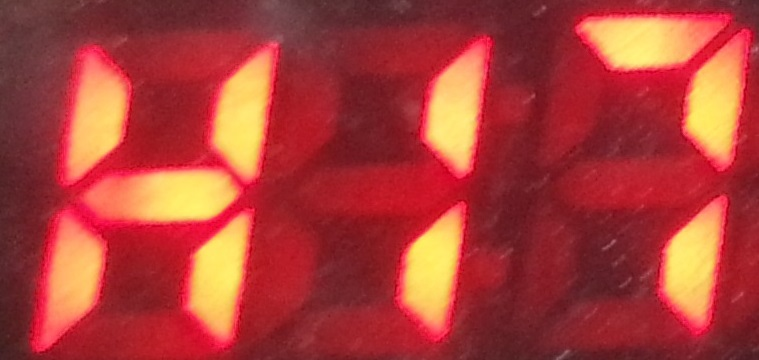
\includegraphics[scale=0.3]{Bilder/ROOMBA_HIT}
	\end{center}
	\item BIG DADY: Wird als großer Panzer auf dem Display des Karts angezeigt:
	
	\begin{center}
		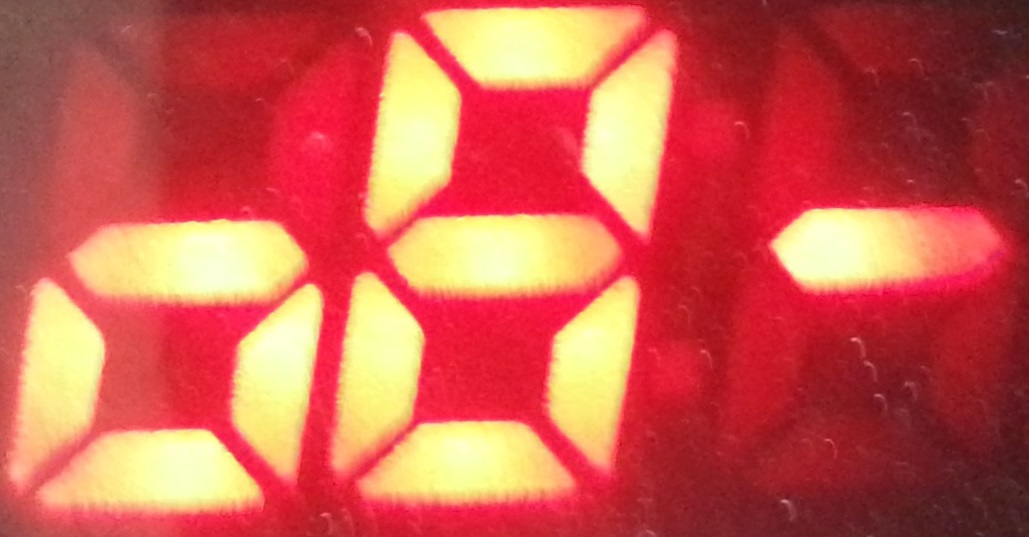
\includegraphics[scale=0.2]{Bilder/BIG_DADY}
	\end{center}
	
	Wirkung: Wenn dieses Powerup aktiviert wird, besteht ein sieben Sekunden Schutz vor  
	dem Powerup RED TANK. 
	\item MUSHROOM: Wird als Pilz auf dem Display des Karts angezeigt. 
	
	\begin{center}
		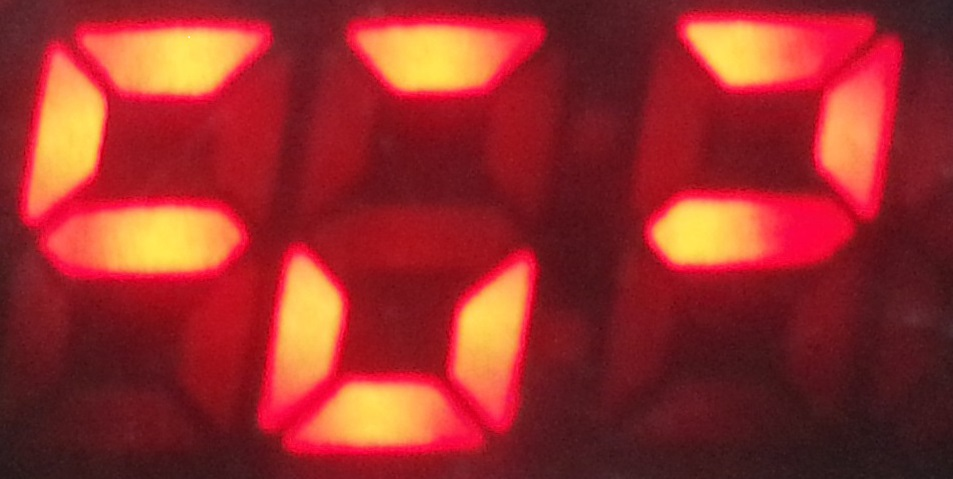
\includegraphics[scale=0.2]{Bilder/MUSHROOM}
	\end{center}
	
	Wirkung: Kart kann sieben Sekunden ungestraft die Seitenbegrenzung der Strecke verlassen. 		
	Wenn der Kurs verlassen wurde, aber nicht rechtzeitig wieder befahren wird, hat dieser 	
	Spieler das Rennen verloren und das Kart bleibt stehen.
\end{itemize}

Der Gewinner des Spiels bekommt anschließend bei einer feierlichen Zeremonie das goldene Klebeband verliehen. 


 



































